\documentclass[11pt]{article}
\usepackage{amsmath}
\usepackage{geometry}
\usepackage{booktabs}
\usepackage{fancyhdr}
\usepackage{graphicx}
\usepackage{listings}
\usepackage{xcolor}
\usepackage{titlesec}
\titleformat{\section}{\normalfont\large\bfseries}{\thesection}{1em}{}
\titleformat{\subsection}{\normalfont\normalsize\bfseries}{\thesubsection}{1em}{}

\definecolor{codegreen}{rgb}{0,0.6,0}
\definecolor{codegray}{rgb}{0.5,0.5,0.5}
\definecolor{codepurple}{rgb}{0.58,0,0.82}
\definecolor{backcolour}{rgb}{0.95,0.95,0.92}

\lstdefinestyle{mystyle}{
  backgroundcolor=\color{backcolour},
  commentstyle=\color{codegreen},
  keywordstyle=\color{magenta},
  numberstyle=\tiny\color{codegray},
  stringstyle=\color{codepurple},
  basicstyle=\ttfamily\footnotesize,
  breakatwhitespace=false,
  breaklines=true,
  captionpos=b,
  keepspaces=true,
  numbers=left,
  numbersep=5pt,
  showspaces=false,
  showstringspaces=false,
  showtabs=false,
  tabsize=2
}

\lstset{style=mystyle}
\geometry{a4paper, margin=1in}
\setlength{\parindent}{0pt}
\setlength{\parskip}{0.5em}
\setlength{\headheight}{15pt}

\pagestyle{fancy}
\fancyhf{}
\lhead{Spring 2026 Intro to Deep Learning}
\rhead{Homework Assignment 3}
\rfoot{Page \thepage}

\begin{document}

\begin{center}
  {\Large \textbf{Homework Assignment 3}} \\
  \vspace{0.2cm}
  \textbf{Due Date:} March 23, 2026 \\
  \textbf{Name:} Karim Smires
\end{center}
\hrule
\vspace{0.5cm}

\section*{Part (a) --- PyTorch (Mandatory)}

\subsection*{Hyperparameters}
\begin{table}[h]
  \centering
  \begin{tabular}{ll}
    \toprule
    \textbf{Hyperparameter} & \textbf{Value} \\
    \midrule
    Optimizer     & Adam \\
    Learning rate & 0.001 \\
    Batch size    & 128 \\
    Epochs        & 15 \\
    \bottomrule
  \end{tabular}
\end{table}

\subsection*{Training Output}
\begin{center}
  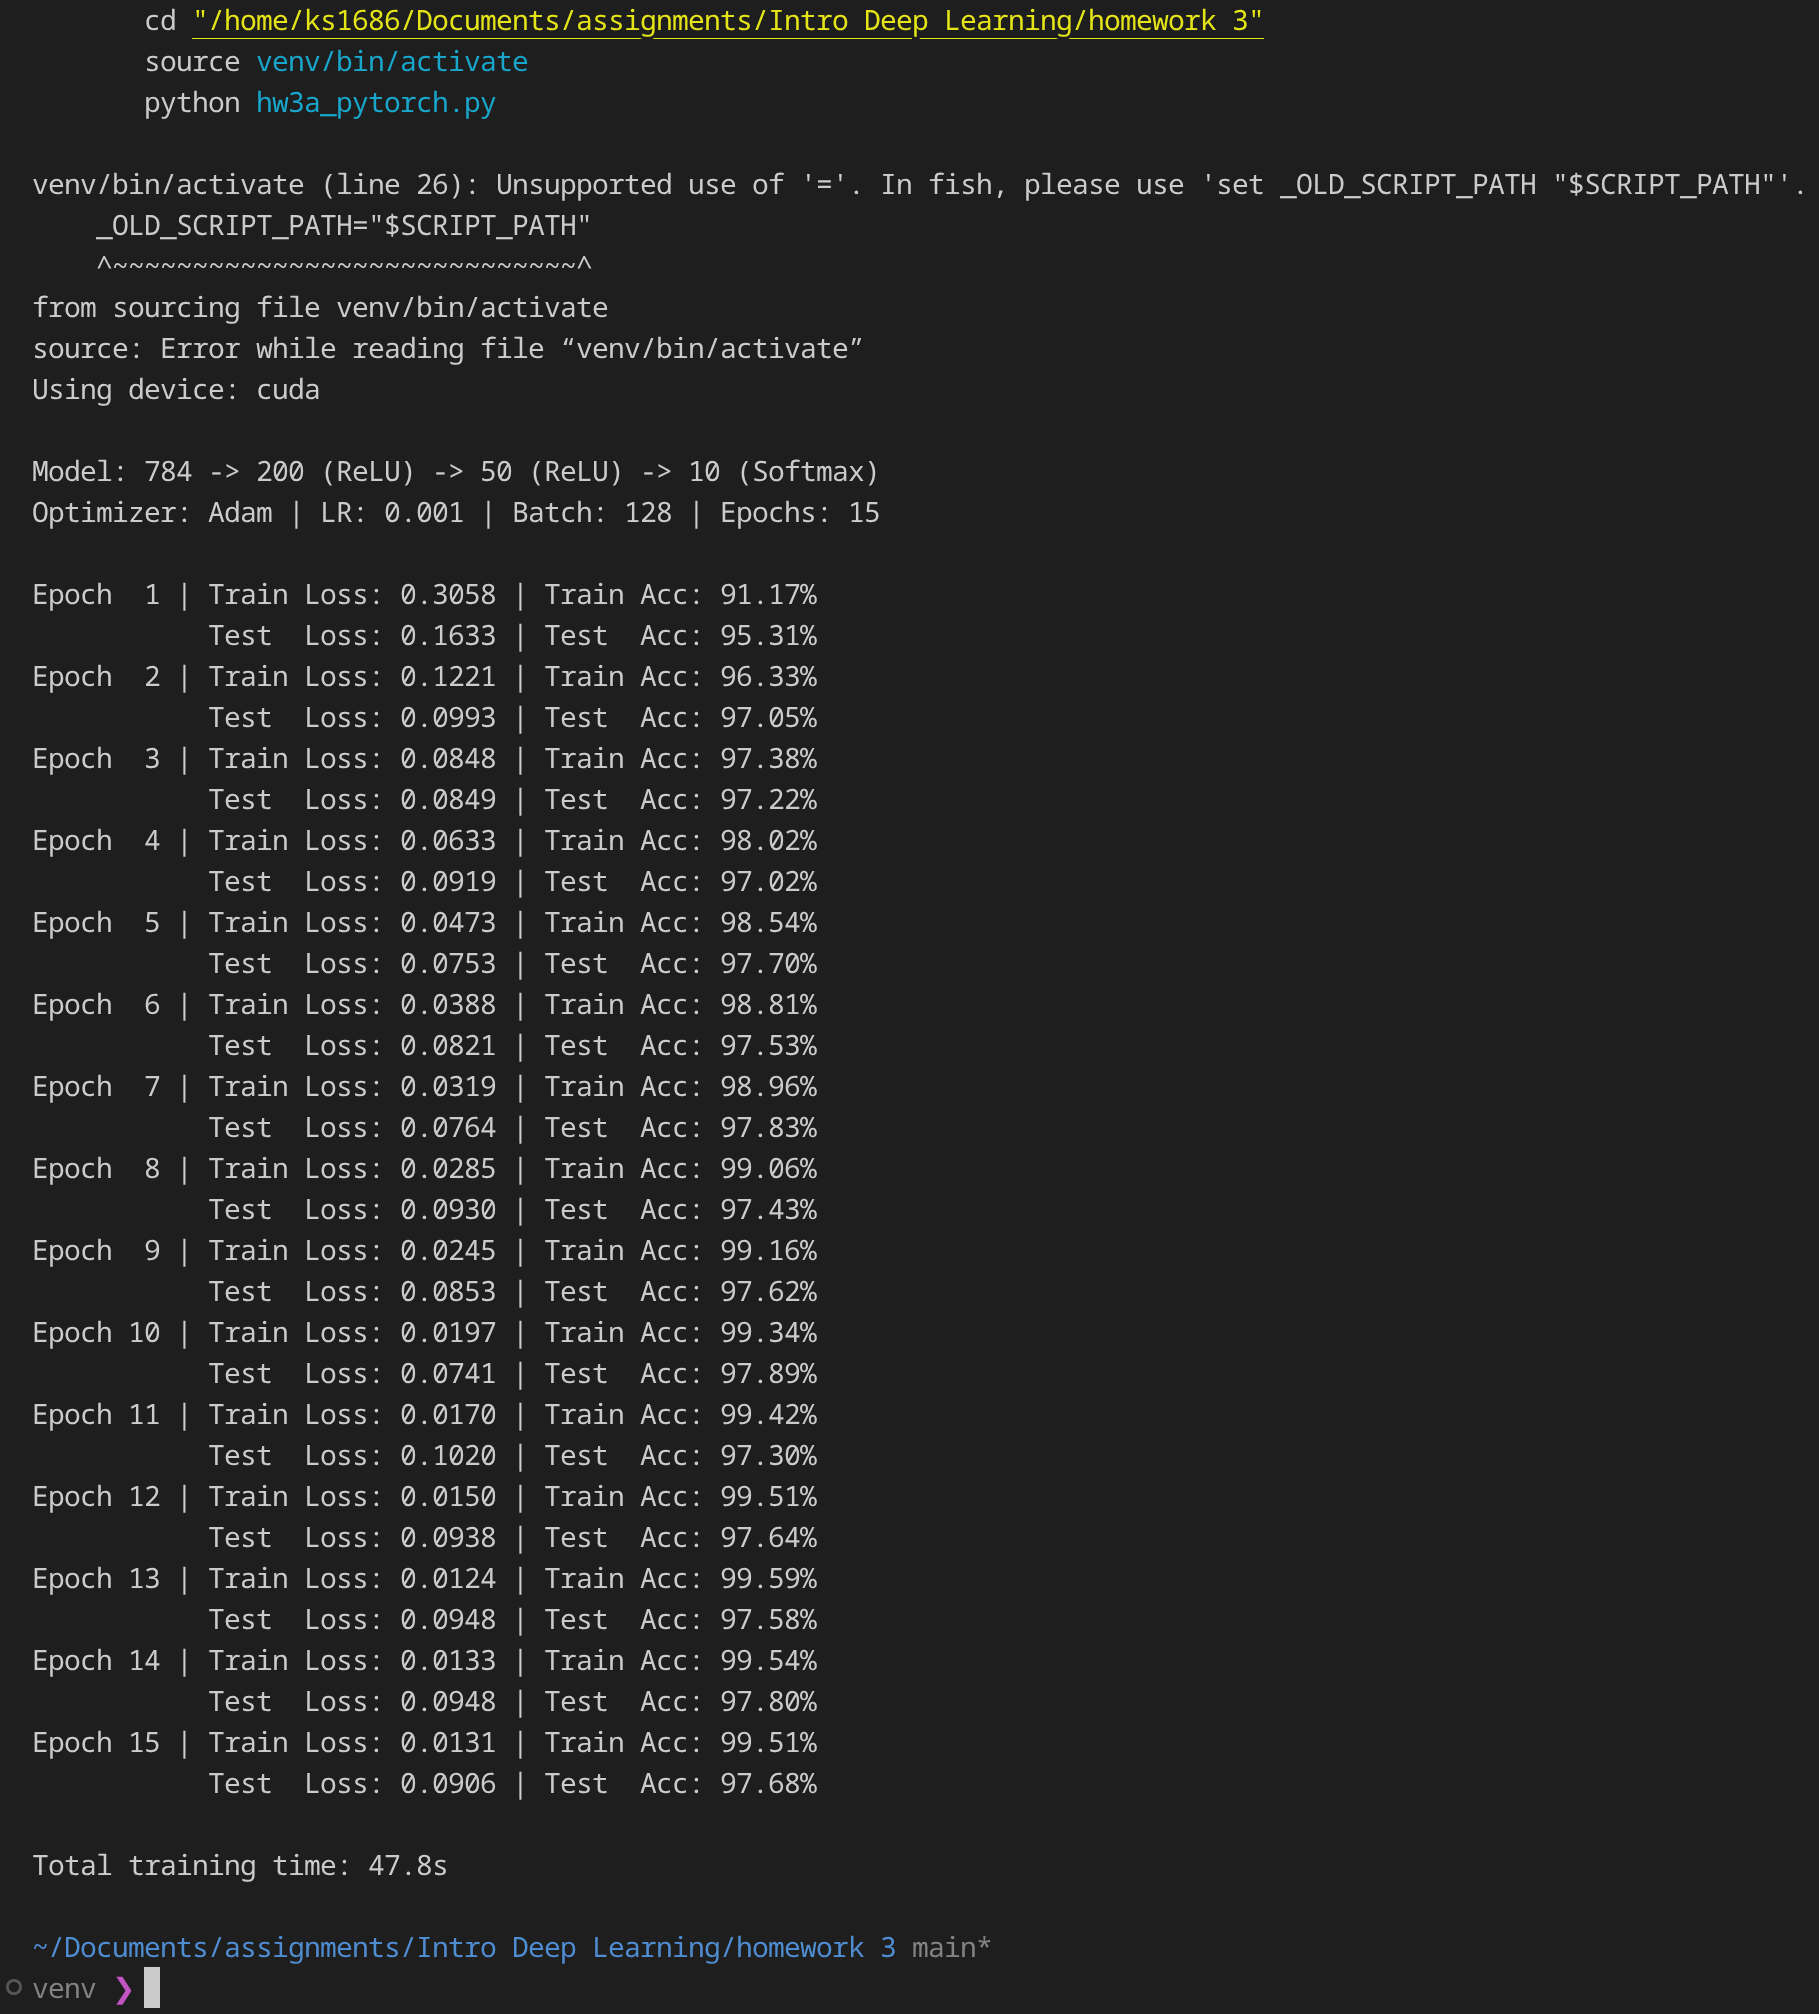
\includegraphics[width=0.74\textwidth]{hw3a_output.png}
\end{center}

\subsection*{Source Code}
\lstinputlisting[language=Python, caption=hw3a\_pytorch.py]{../hw3a_pytorch.py}

\vspace{0.5cm}
\hrule
\vspace{0.5cm}

\section*{Part (b) --- NumPy Only (Optional)}

\subsection*{Hyperparameters}
\begin{table}[h]
  \centering
  \begin{tabular}{ll}
    \toprule
    \textbf{Hyperparameter} & \textbf{Value} \\
    \midrule
    Optimizer     & Mini-batch SGD \\
    Learning rate & 0.01 \\
    Batch size    & 128 \\
    Epochs        & 20 \\
    \bottomrule
  \end{tabular}
\end{table}

\subsection*{Training Output}
\begin{center}
  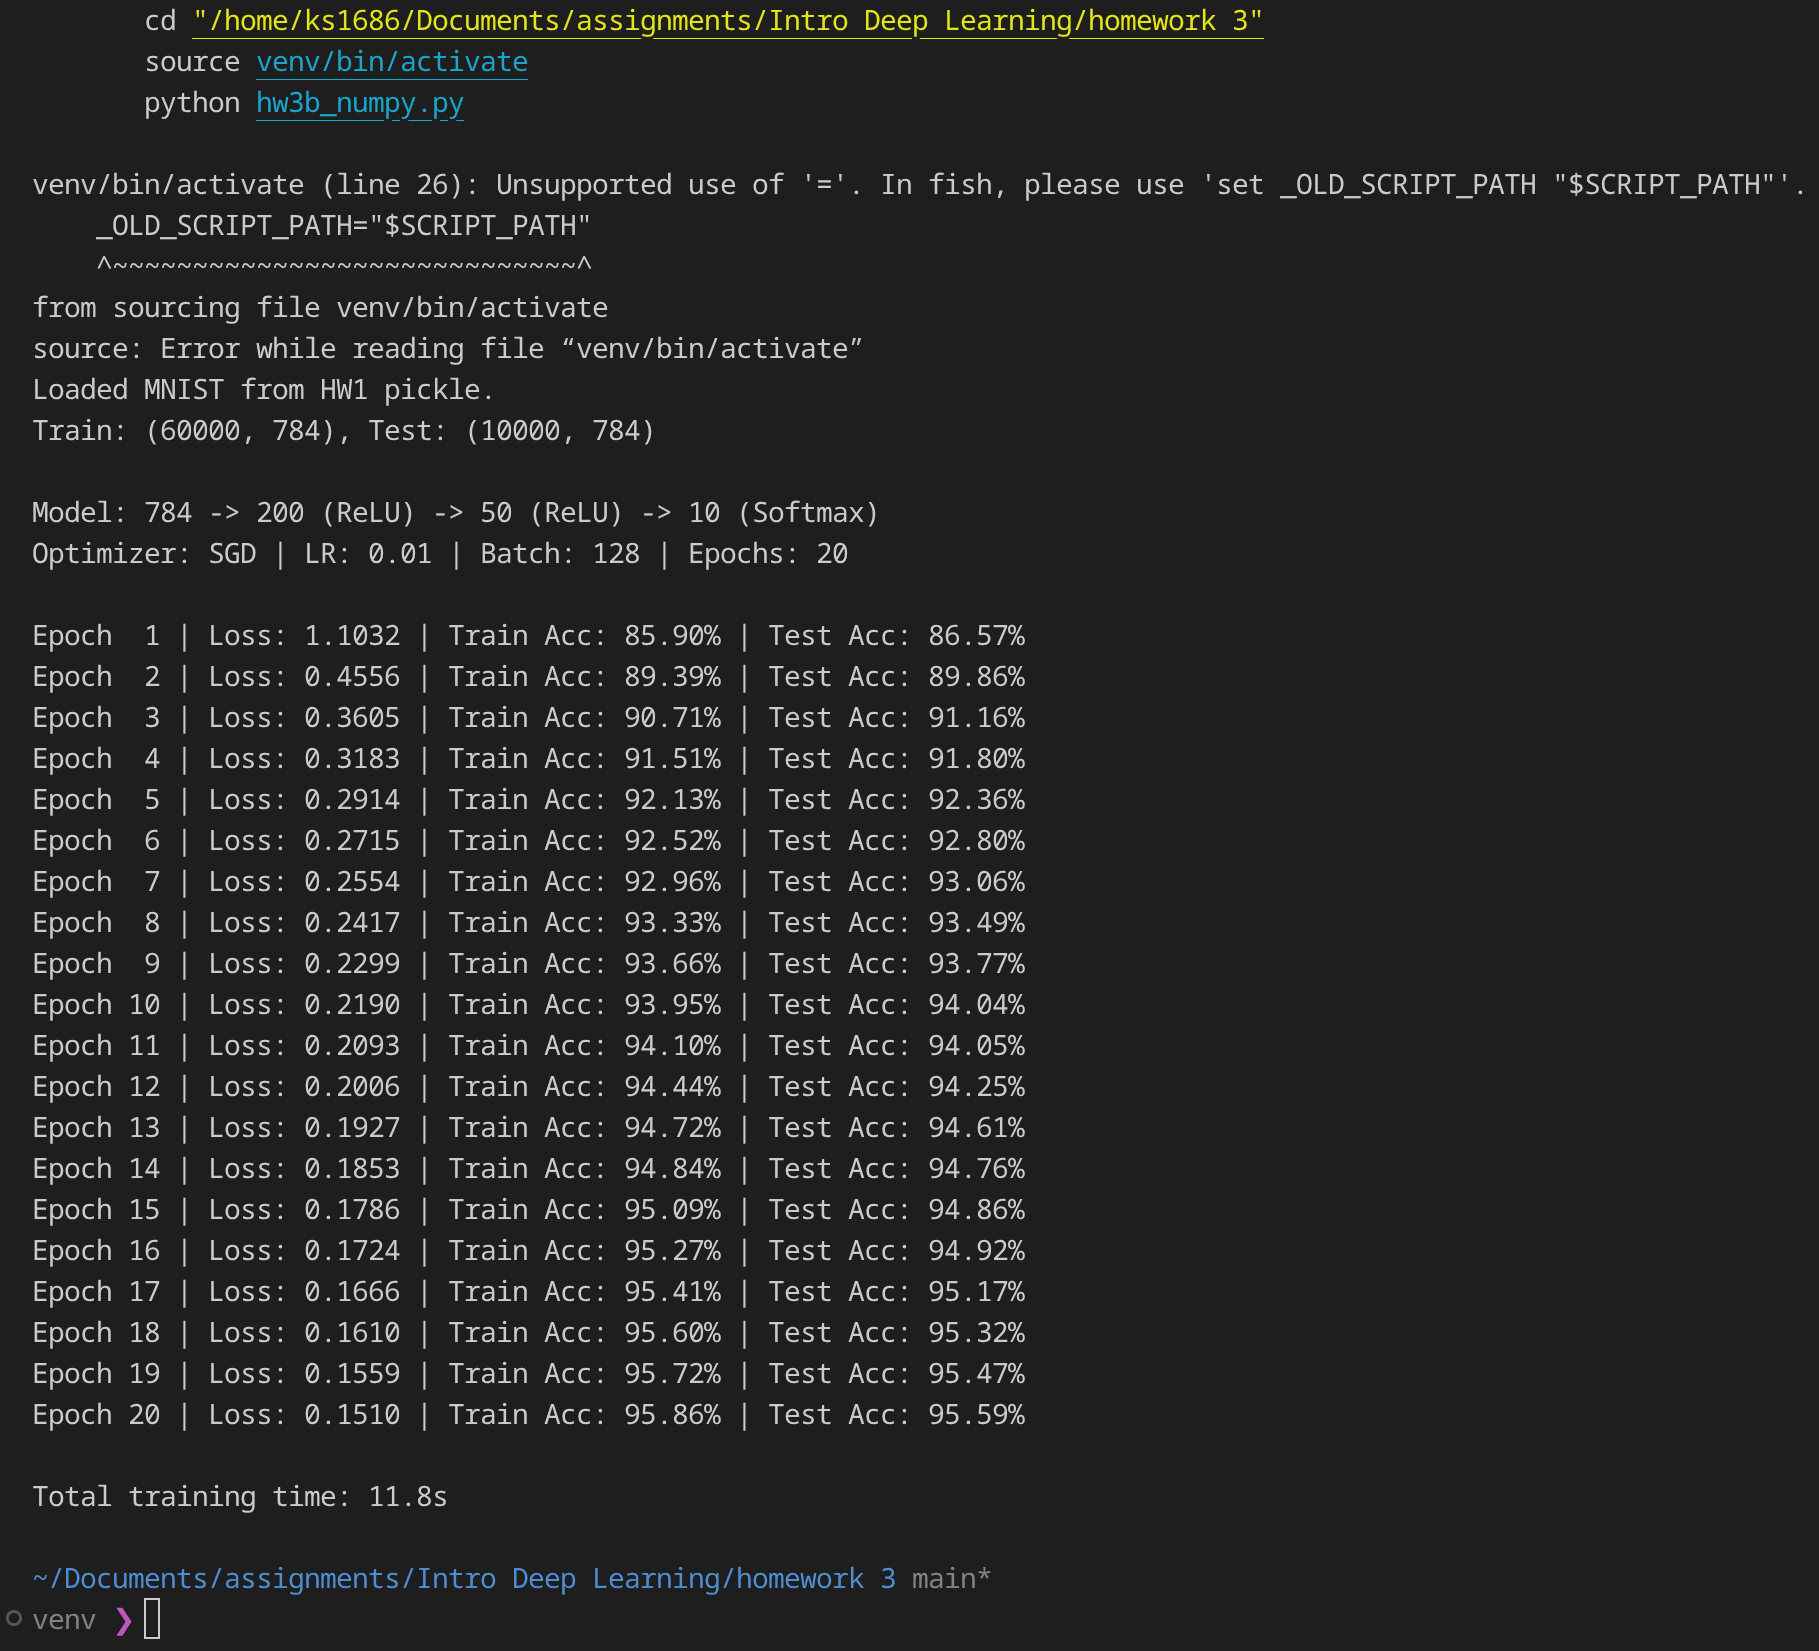
\includegraphics[width=0.74\textwidth]{hw3b_output.png}
\end{center}

\subsection*{Source Code}
\lstinputlisting[language=Python, caption=hw3b\_numpy.py]{../hw3b_numpy.py}

\vspace{0.5cm}
\hrule
\vspace{0.5cm}

\section*{Summary}

\begin{table}[h]
  \centering
  \begin{tabular}{lcccc}
    \toprule
    \textbf{Implementation} & \textbf{Optimizer} & \textbf{Train Acc} & \textbf{Test Acc} & \textbf{Time} \\
    \midrule
    Part (a) PyTorch (GPU) & Adam, LR=0.001, 15 ep & 99.64\% & 97.99\% & 38.7 s \\
    Part (b) NumPy (CPU)   & SGD,  LR=0.01,  20 ep & 95.86\% & 95.59\% & 19.7 s \\
    \bottomrule
  \end{tabular}
  \caption{Both implementations exceed the 95\% test accuracy requirement.}
\end{table}

\end{document}
